\documentclass{article}
\usepackage{hyperref}
\usepackage{amsmath}
\usepackage{amssymb}
\usepackage{pgfplots}
\usepackage{float}
\usepackage{todonotes}
\usepackage{tikz}
\usepackage[shortlabels]{enumitem}

\renewcommand{\Re}{\mathbb{R}}
\newcommand{\Li}{\mathcal{L}}
\newcommand{\Ex}{\mathbb{E}}
\renewcommand{\Pr}{\mathbb{P}}
\newcommand{\Hy}{\mathcal{H}}
\newcommand{\sign}{\text{sign}}
\newcommand{\error}{\text{error}}

\newcommand\bigO[1]{
    \ensuremath{\mathcal{O}\left(#1\right)}
    }

\newcommand{\sigmoidPlot}{
    
    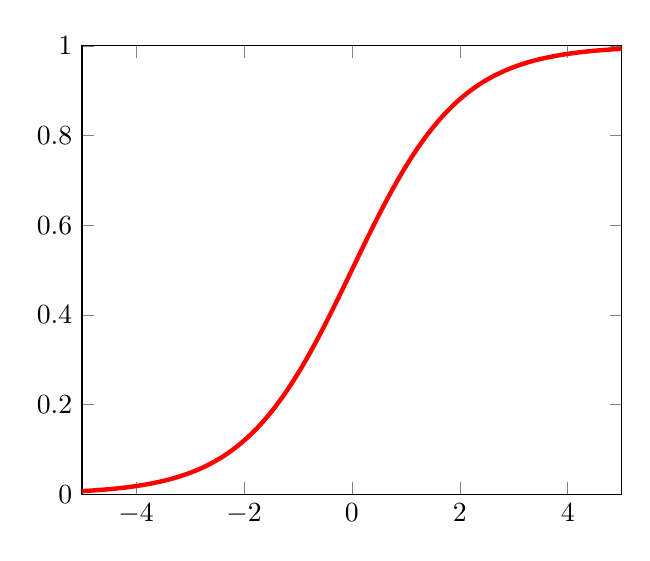
\begin{tikzpicture}
        \begin{axis}[xmin=-5, xmax=5, ymin=0, ymax=1, samples=150]
        \addplot[red, ultra thick] {1/(1+exp(-x))};
        \end{axis}
    \end{tikzpicture}
    
    }

\usetikzlibrary{positioning, calc}
\usetikzlibrary{arrows.meta}

\tikzstyle{circlebox}=[circle,thick,draw=black!75,minimum size=8mm]
\tikzstyle{inputnode}=[circlebox, draw=blue!75]
\tikzstyle{hiddennode}=[circlebox, draw=orange!75]
\tikzstyle{outputnode}=[circlebox, draw=orange!75]
\tikzstyle{simplebox}=[rectangle,thick,draw=black!75,
fill=black!20,minimum size=4mm]
\tikzstyle{textbox}=[rectangle,thick,minimum size=4mm,draw=black!0,
fill=black!0]
\tikzstyle{halfvdistance}=[yshift=-0.7cm]
\tikzstyle{abovebetween}=[xshift=-2.7mm]
\tikzstyle{edgepath} = [-Latex,->,shorten >=1pt,-stealth,semithick, rounded 
corners=5pt]

\def \nodedv {0.735cm}
\def \nodedh {0.65cm}

\tikzset{
    between/.style args={#1 and #2}{
        at = ($(#1)!0.5!(#2)$)
    }
}

\begin{document}
    \section{Subjects}
    \begin{itemize}
        \item VC Dimension
        \item Bias Variance
        \item Regularization
        \item Validation
    \end{itemize}
    \section{Notes}
    
    \subsection{Preceding discussion}
    \textit{Chapter 2 in Learning from data.}\\
    What we want to minimize, is the out-of-sample error:
    \begin{equation*}
    E_{out}(g) = \Ex_{x,y}\left(e\left(g(x), y\right)\right)
    \end{equation*}
    We can't minimize this, however what we can minimize is the in-sample-error:
    \begin{equation*}
    E_{in}(g)=\frac{1}{\|D\|} \sum_{(x,y) \in D} e\left(g(x), y\right)
    \end{equation*}
    So we are hoping, or aiming for, that the generalization error 
    $E_{in}-E_{out}$ should be small, so when we minimize $E_{in}$ it benefits 
    $E_{out}$.\\
    Recall that the Hoeffding inequality provides a way to bound the 
    generalization error:
    \begin{equation*}
    \Pr[|E_{in}(g) - E_{out}(g)| > \epsilon] \leq 2Me^{-2\epsilon^2N}
    \end{equation*}
    We can rephrase this, by introducing a tolerance level $\delta$ and assert 
    with probability at least $1 - \delta$ that: 
    \begin{equation*}
    E_{out}(g) \leq E_{in}(g) + \sqrt{\frac{1}{2N}\ln\frac{2M}{\delta}}
    \end{equation*}
    We notice here, that the bound depends on $M$, which is the size of the 
    hypothesis set. Unfortunately, most problems has infinite hypotheses, and 
    thus the bound will become meaningless as it goes towards infinity. So we 
    want to replace $M$ by something that stays meaningful as $M$ goes to 
    infinity. 
    
    To this end we introduce the growth function, which will formalize the 
    effective number of hypotheses. Furthermore, a \textit{dichotomy} is an 
    $N$-tuple, generated by a hypothesis, which splits the data into two 
    groups.
    
    The set of dichotomies generated by the hypothesis set $\Hy$ on the points 
    $x_1,\dots,x_n$ is defined by:
    \begin{equation}
    \Hy(x_1,\dots,x_N)= \{(h(x_1),\dots,h(x_N)) \,|\, h \in \Hy)\}
    \end{equation}
    One can think of the dichotomies as being the hypothesis set as seen 
    through the eyes of just $N$ points. We can then define the growth function 
    as:
    \begin{equation}
    m_\Hy(N)=\max\limits_{x_1, \dots, x_n \in X} |\Hy(x_1,\dots, x_N)|
    \end{equation}
    I.e. the maximum number of dichotomies that can be generated by $\Hy$ on 
    any $N$ points. If we just look at binary classification, then the upper 
    limit on the amount of dichotomies for a data-set of size $N$ is: 
    \begin{equation}
    m_\Hy(N) \leq 2^N
    \end{equation}
    If $\Hy$ is capable of generating all possible dichotomies on the data-set, 
    then $m_\Hy(n) = 2^N$ and we say that $\Hy$ shatter $x_1,\dots,x_n$. If 
    there is no such data-set of size $k$ that can be shattered by $\Hy$ then 
    we say that $k$ is a breakpoint for $\Hy$.
    
    If there is such a breakpoint $k$, then we know that $m_\Hy(k) < 2^N$. We 
    define $B(N,k)$ as the maximum number of dichotomies on $N$ points, such 
    that no subset of size $k$ can be shattered by these dichotomies. We can 
    then see that:
    
    \begin{equation*}
    m\Hy(N) \leq B(N,k)\, \text{ if $k$ is a break point for }\Hy
    \end{equation*}
    
    Sauer's lemma then states that:
    \begin{equation*}
    B(N,k) \leq \sum_{i=0}^{k-1}\begin{pmatrix}
    N\\
    i
    \end{pmatrix}
    \end{equation*}
    
    Which means that:
    \begin{equation*}
        m_\Hy(N) \leq \sum_{i=0}^{k-1} \begin{pmatrix}
        N\\i
        \end{pmatrix}
    \end{equation*}
    
    We then see that, if $\Hy$ has a breakpoint then $m_\Hy(N)$ has a 
    polynomial bound. This is important because when $m_\Hy(N)$ has a 
    polynomial bound, the generalization error will go to zero as $N 
    \rightarrow \infty$
    
    \subsection{VC Dimension}
    The Vapnik-Chervonenkis dimension of a hypothesis set $\Hy$, denoted by 
    $d_{vc}(\Hy)$ or simply $d_{vc}$ is the largest value of $N$ for which 
    $m_\Hy(N)=2^N$. If $m_\Hy(N)=2^N$ for all $N$, then $d_{vc}(\Hy)=\infty$.
    
    It follows then, that if $d_{vc}$ is the VC dimension for $\Hy$, then $k = 
    d_{vc} + 1$ is a breakpoint and there are no smaller breakpoints. We can 
    therefore rewrite the previous sum in terms of the VC dimension:
    
    \begin{equation*}
        m_\Hy(N) \leq \sum_{i=0}^{d_{vc}} \begin{pmatrix}
        N\\i
        \end{pmatrix}
    \end{equation*}
    
    We then arrive at the VC Generalization Bound:
    \begin{equation}
        E_{out}(g) \leq E_{in}(g) + \sqrt{\frac{8}{N} \ln 
        \frac{4m_\Hy(2N)}{\delta}}
    \end{equation}
    with probability $\geq 1-\delta$
    
    VC-Dimension captures expressiveness/capacity of hypothesis spaces and 
    relate them to generalization. Leads to out-of-sample error equals 
    in-sample-error + model complexity:
    \begin{equation*}
    E_{out}(h) \leq E_{in}(h) + \Omega(N,\Hy, \delta)
    \end{equation*}
    \begin{equation*}
    \Omega(N, \Hy, \delta) = \sqrt{\frac{8}{N}\ln\frac{4m_\Hy(2N)}{\delta}}
    \end{equation*}
    \todo{Sampling	Complexity}
    
    \subsection{Bias-Variance decomposition}
    \textit{Page 62}\\
    The out-of-sample error for hypothesis $g^{(D)}$ learned on data $D$ is:
    \begin{equation*}
        E_{out}(g^{(D)}) = \Ex_x\left[(g^{(D)}(x)-f(x))^2\right]
    \end{equation*}
    Where $\Ex_x$ denotes the expected value with respect to $x$ (based on the 
    probability distribution on the input space $X$)
    
    We can generalize this, to remove the dependence on a specific data-set by 
    taking the expectation with respect to all data-sets:
    \begin{align*}
        \Ex_D\left[E_{out}(g^{(D)})\right] &=
        \Ex_D\left[\Ex_x\left[(g^{(D)}(x)-f(x))^2\right]\right]\\
            &= \Ex_x\left[\Ex_D\left[(g^{(D)}(x)-f(x))^2\right]\right]\\
            &= \Ex_x\left[\Ex_D\left[g^{(D)}(x)^2\right] - 
            2\Ex_D\left[g^{(D)}(x)\right]f(x)+f(x)^2)\right]
    \end{align*}
    
    The term $\Ex_D\left[g^{(D)}(x)\right]$ gives an 'average function', which 
    we denote by $\bar{g}(x)$ it can be seen as an average function as a result 
    of many data-sets $D_1,\dots,D_K$ where:
    \begin{equation}
        \bar{g}(x)\approx \frac{1}{K} \sum_{k=1}^{K}g_k(x)
    \end{equation}
    
    We can now rewrite the expected out-of-sample error in terms of $\bar{g}$:
    \begin{align*}
        &\Ex_D\left[E_{out}(g^{(D)})\right]\\
        &=\Ex_x\left[\Ex_D\left[g^{(D)}(x)^2\right] - 2\bar{g}(x)f(x)+ 
        f(x)^2\right]\\
        &=\Ex_x\left[\Ex_D\left[g^{(D)}(x)^2\right]-\bar{g}(x)^2 + \bar{g}(x)^2 
        - 2\bar{g}(x)f(x)+f(x)^2\right]\\
        &=\Ex_x\left[\Ex_D\left[(g^{(D)}(x) - \bar{g}(x))^2\right] + 
        (\bar{g}(x)-f(x))^2\right]
    \end{align*}
    
    The term to the right $(\bar{g}(x)-f(x))^2$ measure how much the average 
    function we would learn using the $D$ different data-sets deviates from the 
    target function, we call this term the bias:
    \begin{equation*}
        \text{bias}(x)=(\bar{g}(x)-f(x))^2
    \end{equation*}
    The other term, $\Ex_D\left[(g^{(D)}(x)-\bar{g}(x))^2\right]$ is what we 
    call the variance, which measures the variation in the final hypothesis:
    \begin{equation}
        \text{var}(x)=\Ex_D\left[(g^{(D)}(x)-\bar{g}(x))^2\right]
    \end{equation}
    We thus arrive at the bias-variance decomposition of out-of-sample error:
    \begin{align*}
        \Ex_D\left[E_{out}(g^{(D)})\right] &= \Ex_x\left[\text{bias}(x) + 
        \text{var}(x)\right]\\
            &= \text{bias} + \text{var}\\
        \text{bias} &= \Ex_x\left[\text{bias(x)}\right]\\
        \text{var} &= \Ex_x\left[\text{var(x)}\right]
    \end{align*}
    \textit{Bias:} How well can we actually fit - on average\\
    \textit{Variance:} How much will data samples lead me astray - on average
    
    We cannot compute actual bias and variance in practice, since they depend 
    on the target function and input probability distribution. So it is a 
    conceptual tool, which is helpful when it comes to developing a model.
    
    There are two typical goals: we want to reduce the variance without 
    significantly increasing bias et vice versa. These goals are achieved 
    through heuristics, regularization being one them.
    
    \textbf{Intuition}
    The bias term is big if the model has too little capacity to fit the data.
    
    The variance term is big if the model has so much capacity, that it is good 
    at fitting noise (sampling errors) in any training set.
    
    \subsection{Regularization}
    In learning, we want to achieve two things:
    \begin{enumerate}
        \item Ensure that out-of-sample error is close to in-sample-error \\
        $\Pr\left[|E_{in} - E_{out}| > \epsilon\right] \leq 
        2Me^{-2\epsilon^2N}$ or:\\
        $E_{out}(h)\leq E_{in}(h)+\Omega(N,\Hy,\delta)$ 
        \item Minimize in-sample-error $E_{in}$
    \end{enumerate}
    So far we have looked at how to prevent underfitting, i.e. how do we fit 
    our data as well as possible. Regularization is about preventing 
    over-fitting, i.e. if we fit our data really well, then our in-sample-error 
    might be really low $E_{in}=0$, but it's no longer close to the 
    out-of-sample-error $E_{out}>>E_{in}$
    
    This happens because we fit the noise rather than the signal, if we look at 
    the target complexity, e.g. for some polynomial, then if we try to fit it 
    with a hypothesis of $h_{10}$, then as the target complexity increases 
    there will be more and more data that our hypothesis cannot capture, so 
    even though it is not stochastic noise, it wil look like noise to our 
    hypothesis. This is reflected in the fact that:
    \begin{itemize}
        \item Data increases $\rightarrow$ Overfitting Decreases
        \item Noise increases $\rightarrow$ Overfitting Increases
        \item Target Complexity Increases $\rightarrow$ Overfitting Increases
    \end{itemize}
    So increasing the target complexity seems to introduce noise similar to 
    increasing the noise. In order to avoid this, we want to fit it in a 
    ``simpler'' way, so we avoid the precise fitting we get from our current 
    techniques.
    
    In linear regression, this is what we currently minimize:
    \begin{equation*}
        E_{in} = \frac{1}{|D|} \sum_{x,y \in D}(w^Tx-y)^2
    \end{equation*}
    If we instead, for different values of $\alpha$, minimize:
    \begin{equation*}
    E_{in}+\Omega(h) = \frac{1}{|D|} \sum_{x,y \in D}(w^Tx-y)^2 + 
    \alpha\|w\|^2_2
    \end{equation*}
    
    Which gives us the constrained optimization:
    \begin{align*}
        \text{Minimize: }&\frac{1}{|D|}\sum_{x,y \in D} (w^Tx - y)^2\\
        \text{Subject to: }&\lambda\|w\|^2_2\leq C
    \end{align*}
    Then we get the constrained hypothesis set $\Hy_{\text{Constrained}}$ where:
    \begin{equation*}
        \Hy_\text{Constrained} \subseteq \Hy \implies 
        d_{vc}(\Hy_\text{Constrained}) \leq d_{vc}(\Hy)
    \end{equation*}
    So we get a simpler hypothesis set (even though $d_{vc}$ might be the 
    same), which also means the variance should go down (as the regularization 
    favors $h$'s that look alike, and rules out the ones that are specialized 
    to a single data-set) although the bias should go up.\todo{why?}
    
    Then for e.g. linear regression we get that:
    \begin{equation*}
        \nabla_w=\frac{1}{n}(2X^TXw-2X^Ty) + \frac{\lambda w}{2n}
    \end{equation*}
    Which gives us that:
    \begin{equation*}
        w = (X^TX+\lambda I)^{-1}X^Ty
    \end{equation*}
    
    For gradient descent, we get that when we minimize $E_{in} + \lambda 
    \|w\|^2_2$, the gradient descent step that previously looked like:
    \begin{equation*}
        w_{t+1} = w_t - \alpha \nabla_w f(w_t)
    \end{equation*}
    will now become:
    \begin{align*}
        w_{t+1} &= w_t - \alpha \nabla_w E_{in}(w_t) - 2 \alpha \lambda w_t\\
            &= w_t(1-2 \alpha \lambda) - \alpha \nabla_w E_{in}(w_t)
    \end{align*}
    Thus, every round the $(1-2\alpha \lambda)$ factor will make $w$ decay 
    towards the zero vector.
    
    \subsection{Validation}
    Regularization introduces the need for validation in order to be able to 
    train on the data again and again with different values of $\lambda$. The 
    need for validation becomes apparent without regularization in more 
    advanced models (like Neural Networks) but regularization is the first 
    technique we encounter.
    
    Validation simply means to take out $K$ points from the data-set and use 
    them to validate the result of the training on the remaining $N-K$ points.
    
    Validation has the issue that as you increase $K$, the $E_{val}$ estimate 
    tightens but it also increases, as you has less data to train on so 
    $E_{out}$ increases with smaller $N-K$. Analytically:
    \begin{equation*}
        E_{val} = E_{out} \pm \bigO{\frac{\sigma}{\sqrt{K}}}
    \end{equation*}
    As a rule of thumb: $K=\frac{N}{5}$ (20\% of data). If we validate and try 
    out different models with different $E_{val}(m_i)$, then we can pick the 
    best and retrain on all the data, hoping that the model we chose is still 
    the best.
    
    Usually if we have few hyperparameters, (like $\lambda$) then we can just 
    perform grid search (exhaustively search through a range of parameters). If 
    we have many hyperparameters, we should just do ``random sampling'' and 
    repeatedly search on promising areas.
    
    We do, however risk that we now overfit on the validation parameters. So 
    what we really want is a training set, a validation set \textit{and a test 
    set}! We will usually split the data-set by $50/25/25\%$ or $60/20/20\%$ 
    depending on the application and the data available.
    
    For small $K$ we get that $E_{out}(h_{all}) \approx E_{out}(h_{train})$ and 
    for large $K$ we get $E_{out}(h_{train}) \approx E_{val}(h_{train})$, but 
    we would like to have both of these.
    
    It turns out that setting $K=1$ and computing:
    \begin{align*}
        D_n &= D - \{(x_n, y_n)\}\\
        e_n &= E_{val}(h_{D_n}) = e(h_{D_n}, (x_n), y_n)\\
        E_{cv} &= \frac{1}{N} \sum_{i=1}^{N} e_n
    \end{align*}
    This is hard to analyze, since errors are correlated but it has been used 
    successfully in practice. However, doing this cross-validation is slow, as 
    we have to train $N$ times on $N-1$ points. Therefore we use $K$-Fold Cross 
    Validation:
    \begin{itemize}
        \item Split data in $K$ parts of size $\frac{N}{K}$
        \item Run $K$ rounds of validation with different data-sets of size 
        $N-K$ and take the mean error.
    \end{itemize}
    Usually, we will run for $K=10$ or $K=5$, as we are impatient beings with 
    deadlines.
\end{document}